\documentclass[../resumosRCOM.tex]{subfiles}

\newenvironment{conditions}
  {\par\vspace{\abovedisplayskip}\noindent\begin{tabular}{>{$}l<{$} @{${}={}$} l}}
  {\end{tabular}\par\vspace{\belowdisplayskip}}
 
\begin{document} 
\subsection{Data Link layer functions and services}
\subsubsection{Main functions}
\begin{itemize}
    \item Provide service interface to the network layer.
    \item Eliminate/reduce transmission errors.
    \item Regulate data flow: Slow receivers not swamped by fast senders.
\end{itemize}

\subsubsection{Services provided}
\paragraph{}
\textbf{Principal service: }Transfer data from the network layer on the 
source machine to the network layer on the destination machine.
\paragraph{}
There are three reasonable possibilities that we will consider:
\begin{itemize}
    \item \textbf{Unacknowledged connectionless service: }
    \begin{itemize}
        \item No logical connection is established beforehand or released 
        afterwards.
        \item Transmitter sends independent frames without having 
        the destination machine acknowledge them. 
        \item If a frame is lost due to noise on the line, no attempt 
        is made to detect or recover from that loss.
        \item Appropriate when the error rate is very low and for 
        real-time traffic.
    \end{itemize}
    
    \item \textbf{Acknowledged connectionless service: }
    \begin{itemize}
        \item No logical connections used.
        \item Each frame sent is individually acknowledged so the 
        sender knows if a frame arrived correctly or has been lost.
        \item If it has not arrived within a specified time interval, 
        it can be sent again.
        \item This service is useful over unreliable channels, 
        such as wireless systems.(i.e. Wi-Fi).
    \end{itemize}
    
    \item \textbf{Acknowledged connection-oriented service: }
    \begin{itemize}
        \item The source and destination machines establish a connection 
        before any data are transferred.
        \item Each frame is numbered, and the data link layer guarantees 
        that each frame sent is indeed received.
        \item Guarantees that each frame is received exactly once and 
        that all frames are received in the right order.
        \item Appropriate over long, unreliable links (satellite channel,
         long-distance telephone circuit).
        \item Divided in 3 phases:
        \begin{itemize}
            \item \textbf{First phase: }The connection is established 
            (initialize variables and counters needed to keep track of
            which frames have been received and which ones have not).
            \item \textbf{Second phase: } One or more frames are actually 
            transmitted.
            \item \textbf{Third phase: } The connection is released (free
            the variables, buffers, and other resources used to maintain 
            the connection).
        \end{itemize}
    \end{itemize}
\end{itemize}

\subsection{Framing}
\paragraph{}
Breaking up the bit stream into discrete frames, computing a short token called a
checksum for each frame, and including the checksum in the frame when it is 
transmitted.
When a frame arrives at the destination,the checksum is recomputed. 
If it is different from the one contained in the frame, the data link layer
knows that an error occurred.
\paragraph{}
A good design must make it easy for a receiver to find the start of new frames
while using little of the channel bandwidth. We will look at three methods:

\subsubsection{Byte count}
\paragraph{}
Uses a field in the header to specify the number of bytes in the 
frame. When the data link layer at the destination sees the byte count,
it knows how many bytes follow and hence where the end of the frame is.

\paragraph{}
Issues
\begin{itemize}
    \item The count can be garbled by a transmission error.     
    \item A single bit flip, may trigger the destination to get
    out of synchronization. 
    \item If an out-of-sync occurs it is unable to locate the correct
    start of the next frame.
\end{itemize}

\begin{figure}[h]
    \centering
    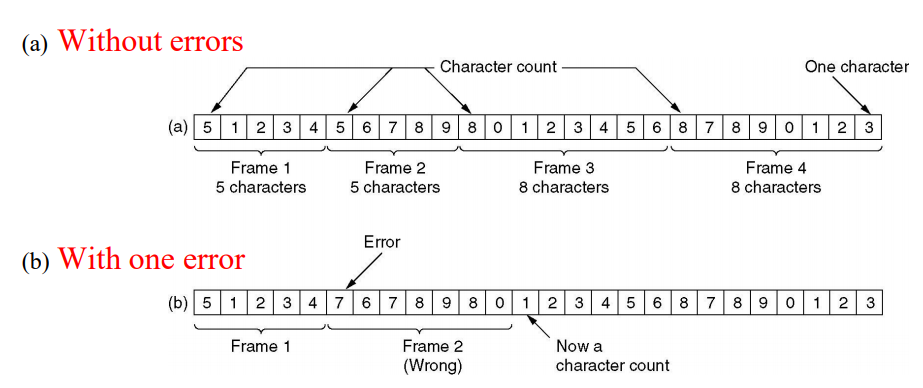
\includegraphics[width=10cm]{byte-count.png}
\end{figure}

\subsubsection{Flag bytes with byte stuffing}
\paragraph{}
This method gets around the problem of resynchronization by having each frame
start and end with special bytes (flag bytes).

\paragraph{}
However, this flag may occur in the middle of the data and induce the receiver
in error by thinking the end of the frame was reached. This issue can be solved
using \textbf{byte stuffing}.

\paragraph{}
\textbf{Byte Stuffing}
\begin{itemize}
    \item Inserting a special escape byte (ESC) before each flag byte in 
    the data.
    \item Makes framing flag bytes distinguishable from the ones in the data.
    \item Escape bytes present in the data also need to be escaped.
\end{itemize}
 
\begin{figure}[h]
    \centering
    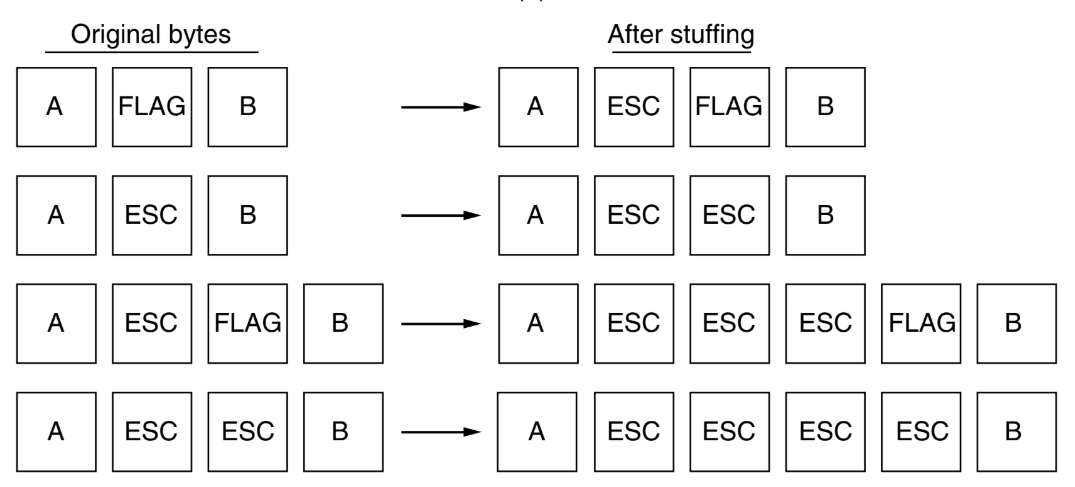
\includegraphics[width=8cm]{byte-stuffing-mechanism.png}
\end{figure}

\subsubsection{Flag bits with bit stuffing}
\begin{itemize}
    \item Each frame begins and ends with a special bit pattern (01111110 / 0x7E).
    \item When the sender finds five consecutive 1 bits in the data, it stuffs a 0 bit
    into the outgoing bit stream.
    \item When the receiver finds five consecutive incoming 1 bits, followed by a 0
    bit, it destuffs the 0 bit.    
\end{itemize}

\paragraph{}
\textbf{Advantages:}
\begin{itemize}
    \item The boundary between two frames is unambiguously recognized by the
    flag pattern (flag sequences can only occur at frame boundaries and never
    within the data).
    \item Frames can contain an arbitrary number of bits made up of units of any
    size.
    \item Ensures a minimum density of transitions that help the physical layer
    maintain synchronization. 
\end{itemize}

\begin{figure}[H]
    \centering
    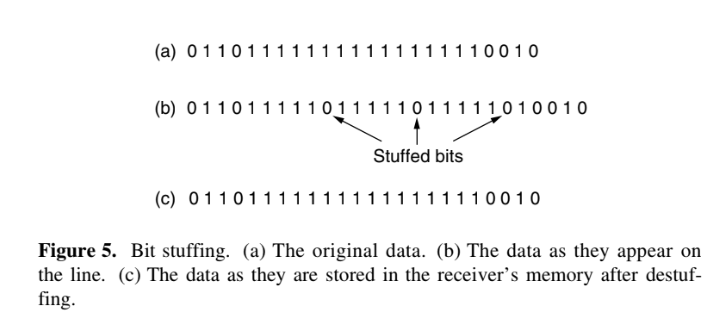
\includegraphics[width=10cm]{bit-stuffing-mechanism.png}
\end{figure}

\paragraph{}
\textbf{Both byte and bit stuffing:}
\begin{itemize}
    \item Are completely transparent to the network layer in both computers.
    \item Have a frame length that depends on the contents of the data.
\end{itemize}

\paragraph{}
Many data link protocols use a combination of these three methods for safety.

\subsection{Error detection}

\subsubsection{Types of Errors}
    \begin{itemize}
        \item \textbf{Simple Error: }Random and independent from previous error.
        \item \textbf{Errors in burst: } 
        \begin{itemize}
            \item Not independent.
            \item Affect neighbour bits.
            \item Burst lenght defined by the first and last bits in error.
        \end{itemize}
    \end{itemize}

\subsubsection{Counting Errors}

\textbf{Frame Error Probability(FER):} 
\begin{equation}
    {FER}= {1-(1- BER)^{n}} 
\end{equation}
\begin{conditions}
    BER & Bit Error Ratio \\
    n & frame length
\end{conditions}
 
\noindent
\newline
\textbf{No Error Probability: } ${P}= (1- p)^{n}$
\newline
\textbf{Error Probability: } ${P}= 1-(1- p)^{n}$ 
\newline
\textbf{i Error Probability: } ${P}= {{n}\choose{i}} p^{i}(1- p)^{n-i}$ 

\begin{conditions}
    p & bit error probability \\ 
    n & frame length \\
\end{conditions}


\subsubsection{Error Detection Techniques}
\paragraph{}
Used by the receiver to determine if a packet contains errors. If a packet is 
found to contain errors, the receiver may request the transmitter to re-send 
the packet.

\subsubsection{Parity Check}

\paragraph{}
\textbf{Simple Parity Check:}
One parity bit added to every k information bits so that:
\begin{itemize}
    \item The total number of bits 1 even (even parity).
    \item The total number of bits 1 odd (odd parity).
\end{itemize}
\paragraph{}
Allows the detection of simple errors and any number of odd errors in a block of 
k + 1 bits. However, does not detect even number of errors in a block of k + 1 bits.

\paragraph{}
\textbf{Bi-dimensional Parity}
\begin{itemize}
    \item Parity per row.
    \item Parity per column.
    \item Minimum code distance = 4.
\end{itemize}

\begin{figure}[H]
    \centering
    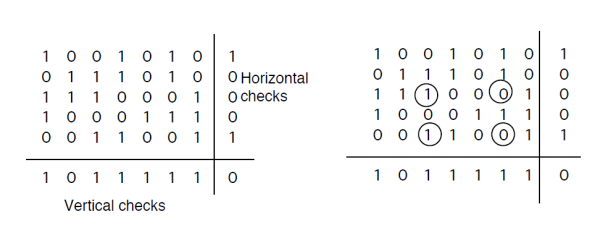
\includegraphics[width=10cm]{bi-dim-parity.png}
\end{figure}


\subsubsection{Cyclic Redundancy Check (CRC)}
\paragraph{}
A fixed number of check bits are appended to the message to be transmitted. 
Data receivers check on the check value attached by finding the remainder of the 
polynomial division of the contents transmitted. If it seems that an error has 
occurred, a negative acknowledgement is transmitted asking for data retransmission.

\begin{figure}[H]
    \centering
    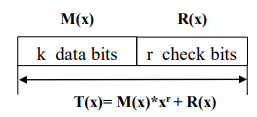
\includegraphics[width=5cm]{CRC-frame.png}
\end{figure}

The bit string is represented as a polynomium (i.e. $110011 \Rightarrow x^5+x^4+x
+1$)

\paragraph{}
\textbf{How to compute the check bits: R(x)?}
\begin{itemize}
    \item Choose a generator string G(x) of length r+1 bits.
    \item Choose R(x) such that T(x) is a multiple of $G(x): T(x)=A\times G(x)$.
\end{itemize}

\paragraph{}
\textbf{Generating R(x):}
\begin{equation}
R(x) = {M(x)x^r}\ \textbf{mod}\ {G(x)}
\end{equation}

\paragraph{}
Choice of G(x) is very important! ($G(x)=x^r+…+1$)

\paragraph{}
\textbf{Generating R(x) example:}
\paragraph{}
Assume for example:
\begin{itemize}
    \item r=3.
    \item $G(x)=x^3 + 1 \Rightarrow 1001$.
    \item $M(x)=x^5+x^4+x^2+1 \Rightarrow 110101$.
\end{itemize}

\paragraph{}
Then:
\begin{itemize}
    \item $x^r = x^3$.
    \item $M(x)\times x^3 = x^8+x^7+x^5+x^3 \Rightarrow 110101000$.
    \item $R(x) = M(x)x^3\ \textbf{mod}\ G(x) = 110101000\ \textbf{mod}\ 1001
    = 011 = x^1 + 1$
\end{itemize}

\paragraph{}
\textbf{Checking at the Receiver}
\begin{itemize}
    \item Divide T(x) by G(x):
    \begin{itemize}
        \item If the remainder $R(x) = 0 \Rightarrow$ no errors.
        \item If the remainder $R(x) != 0 \Rightarrow$ errors have occurred.
    \end{itemize}
\end{itemize}

\paragraph{}
\textbf{Performance:}
\paragraph{}
For r check bits per frame the following can be detected
\begin{itemize}
    \item All patterns of 1, 2, or 3 errors (d > 3).
    \item All bursts of errors of r or fewer bits.
    \item All errors consisting of an odd number of inverted bits.
\end{itemize}


\subsection{Automatic Repeat reQuest (ARQ)}
\paragraph{}
An error-control method for data transmission that uses acknowledgements
(messages indicating whether or not the message has been correctly received)
and timeouts to achieve reliable data transmission over an unreliable service.
This mechanisms automatically request the retransmission of:
\begin{itemize}
    \item Missing packets.
    \item Packets with errors.
\end{itemize}

\paragraph{}
There are three common ARQ schemes:

\subsubsection{Stop and Wait}
\begin{itemize}
    \item  Sender transmits information frame I and waits for positive confirmation
    ACK from receiver.
    \item Receiver receives I frame:
    \begin{itemize}
        \item If I frame has no error sends ACK.
        \item If I frame has error sends NACK.
    \end{itemize}
    \item Sender receives I frame:
    \begin{itemize}
        \item If ACK, proceeds and transmits new frame.
        \item If NACK, retransmits frame I.
    \end{itemize} 
    \item If I, ACK or NACK is lost a timeout is required!
\end{itemize}

\textbf{Issue:}
If the transmitter times-out and sends a packet twice, the receiver cannot tell 
whether the second frame is a retransmission or a new frame transmission.

\textbf{Solution:}
Define a 1 bit sequence number in the header of the frame.

\paragraph{}
This sequence number alternates (from 0 to 1) in subsequent frames. The transmitter sends
a frame with a sequence number attached to it so the receiver can check if it matches the 
expected.  When the receiver sends an ACK, it includes the sequence number of the next 
packet it expects.  This way, the receiver can detect duplicated frames by checking if the
frame sequence numbers alternate.

\paragraph{}
\textbf{Efficiency(S):}
\begin{equation}
    {S}=\frac{T_f}{T_f + 2 \times T_{prop}} = \frac{1}{1+2a}
\end{equation}
where:
\begin{conditions}
   T_f     &   Data transmission time\\
   T_{prop} &  Propagation Delay 
\end{conditions}

\textbf{Probability of k Attempts required to transmit a frame with success} 
\begin{equation}
    {P[A=k]}= {p_e}^{k-1} {(1-p_e)} 
\end{equation}
where:
\begin{conditions}
    p_e & frame error probability(FER)
\end{conditions}

\textbf{Expected number of Attempts to transmit a frame with success} 
\begin{equation}
    {E[A]}= \frac{1}{1-p_e} 
\end{equation}
where:
\begin{conditions}
    p_e & frame error probability(FER)
\end{conditions}

\textbf{Efficiency with Errors} 
\begin{equation}
    {S}= \frac{T_f}{E[A](T_f + 2 \times T_{prop})} = \frac{1-p_e}{1+2a}
\end{equation}
where:
\begin{conditions}
    p_e & frame error probability(FER)
\end{conditions}



\subsubsection{Go Back N}
\paragraph{}
Allows the transmission of new packets before earlier ones are acknowledged.

\paragraph{}
\textbf{Sender:}
\begin{itemize}
    \item May transmit up to W frames without receiving RR(Receiver Ready = ACK).
    \item I frames are numbered sequentially I(NS): I(0), I(1), I(2), etc.
    \item Cannot send I(NS=i+W) until it has received the RR(NR=i).   
\end{itemize}

\paragraph{}
\textbf{Receiver:}
\begin{itemize}
    \item Does not accept frames out of sequence.
    \item Sends RR(NR) to sender indicating:
    \begin{itemize}
        \item That all the packets up to NR-1 have been received in sequence.
        \item The sequence number, NR, of the next expected frame.
    \end{itemize}
\end{itemize}

\paragraph{}
\textbf{Behaviour under Errors}
\begin{itemize}
    \item Frames with errors are silently discarded by the Receiver.
    \item If Receiver receives Data frame out of sequence:
    \begin{itemize}
        \item First out-of-sequence-frame: Receiver sends REJ(NR) where NR =
        next in-sequence frame expected.
        \item Following out-of sequence-frames: Receiver discards them; no REJ
        sent.                
    \end{itemize}
    \item When Sender receives REJ(NR=x), the Sender:
    \begin{itemize}
        \item Goes-Back and retransmits I(x), I(x+1), etc.
        \item Continues using Sliding Window mechanism.
    \end{itemize}
    \item If timeout occurs, the Sender:
    \begin{itemize}
        \item Requests the Receiver to send a RR message.
        \item Sends a special message (RR command message).
    \end{itemize}
\end{itemize}


\paragraph{}
\textbf{Maximum Window Size(W):} 
\begin{equation}
    {W}= {M - 1} = {2^{k} - 1}
\end{equation}
where:
\begin{conditions}
    M & Number of sequence numbers\\
    k & Number of bits used to code sequence numbers \\
\end{conditions}

\paragraph{}
\textbf{Efficiency:}
\begin{itemize}
    \item If $W \geq 1 + 2a \Rightarrow S = 1$.
    \item If $W < 1 + 2a \Rightarrow S = \frac{W}{1 + 2a}$.
\end{itemize}

\paragraph{}
\textbf{Efficiency with Errors:}
\begin{figure}[H]
    \centering
    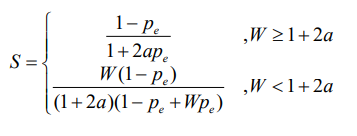
\includegraphics[width=7cm]{go-back-n-eff.png}
    \caption{pe - frame error probability (ratio, FER)}
\end{figure}

\subsubsection{Selective Repeat}
\paragraph{}
Similar to \textbf{Go Back N}, however it does not discard successful frames when errors
occur.

\paragraph{}
\textbf{Receiver:}
\begin{itemize}
    \item Accepts out of sequence frames.
    \item Confirms negatively, SREJ, a frame not arrived.
    \item Uses RR to confirm blocks of frames arrived in sequence.    
\end{itemize}

\paragraph{}
\textbf{Sender:} Retransmits only the frames signaled by SREJ.

\paragraph{}
\textbf{Maximum window size(W):}
\begin{equation}
    {W}= \frac{M}{2} = 2^{k-1}
\end{equation}
where:
\begin{conditions}
    M & Number of sequence numbers\\
    k & Number of bits used to code sequence numbers \\
\end{conditions}

\textbf{Efficiency:}
\begin{figure}[H]
    \centering
    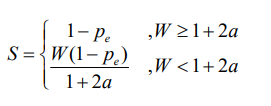
\includegraphics[width=7cm]{selective-repeat-eff.png}
    \caption{pe - frame error probability (ratio, FER)}
\end{figure}

\subsubsection{Useful Formulas for All Methods}

\paragraph{}
\textbf{Data transmission time ($T_f$):}
\begin{equation}
    {T_f}=\frac{L}{R}
\end{equation}
where:
\begin{conditions}
   L     &   Frame Size\\
   R &  Data Rate 
\end{conditions}

\paragraph{}
\textbf{Propagation Delay($T_{prop}$):}
\begin{equation}
    {T_{prop}}=\frac{d}{V}
\end{equation}
where:
\begin{conditions}
   d     &   Distance between sender and receiver \\
   V &  Propagation Velocity
\end{conditions}

\paragraph{}
\textbf{SUMETHIN(a)}
\begin{equation}
    {a}=\frac{T_{prop}}{T_f}
\end{equation}
where:
\begin{conditions}
    T_{prop}    &  Propagation Delay \\
   T_f     &  Data transmission time 
\end{conditions}

\textbf{Maximum Rat($R_{max}$):}
\begin{equation}
    {R_{max}}={S}\times{R}
\end{equation}
where:
\begin{conditions}
   S     &  Efficiency\\
   R &  Data rate
\end{conditions}

\textbf{Round Trip Time(RTT - Time of transmission and acknowledgement of a frame):} 
\begin{equation}
    {RTT}= 2 \times {T_{prop}} + {T_f}
\end{equation}
where:
\begin{conditions}
   T_{prop}     &  Propagation Delay\\
   T_f &   Data transmission time
\end{conditions}

\subsection{Framing, Error detection and ARQ in common networks}
\subsection{Reliability in the Protocol Stack}

\end{document}

